\section{Introduzione}
L'obiettivo di questo elaborato è la presentazione di un approfondimento per l'esame di sicurezza informatica che consiste nell'implementare 
un attacco padding oracle contro un algoritmo di cifratura a blocchi in modalità CBC.
L'algoritmo di cifratura a blocchi scelto è il DES con chiave a 64bit ma potrebbe funzionare anche 
su algoritmi più complessi come AES con chiave a 128bit purchè usati in modalità CBC.
\section{CBC Mode}

CBC (Cipher Block Chaining) è una modalità di cifratura a blocchi, questo significa che il testo in chiaro viene cifrato passando blocchi di bytes di una 
lughezza predefinita alla funzione di cifratura. Se però ogni blocco fosse cifrato indipendentemente senza ulteriori manipolazioni uno stesso 
input genererebbe uno stesso cifrato in output, per questo nella modalità CBC (figura \ref{fig:cbc_enc}), i blocchi non sono cifrati indipendentemente ma 
l'output della cifratura del blocco precedente viene messo in Xor con il testo in chiaro da cifrare generando molta più differenza fra gli output.
visto che è sempre necessario un secondo vettore in input all'inizio è necessario utilizzare un vettore di inizializzazione (IV) random o fisso, in questo progetto viene usato 
un vettore di inizializzazione random.
\begin{figure}[h!]
    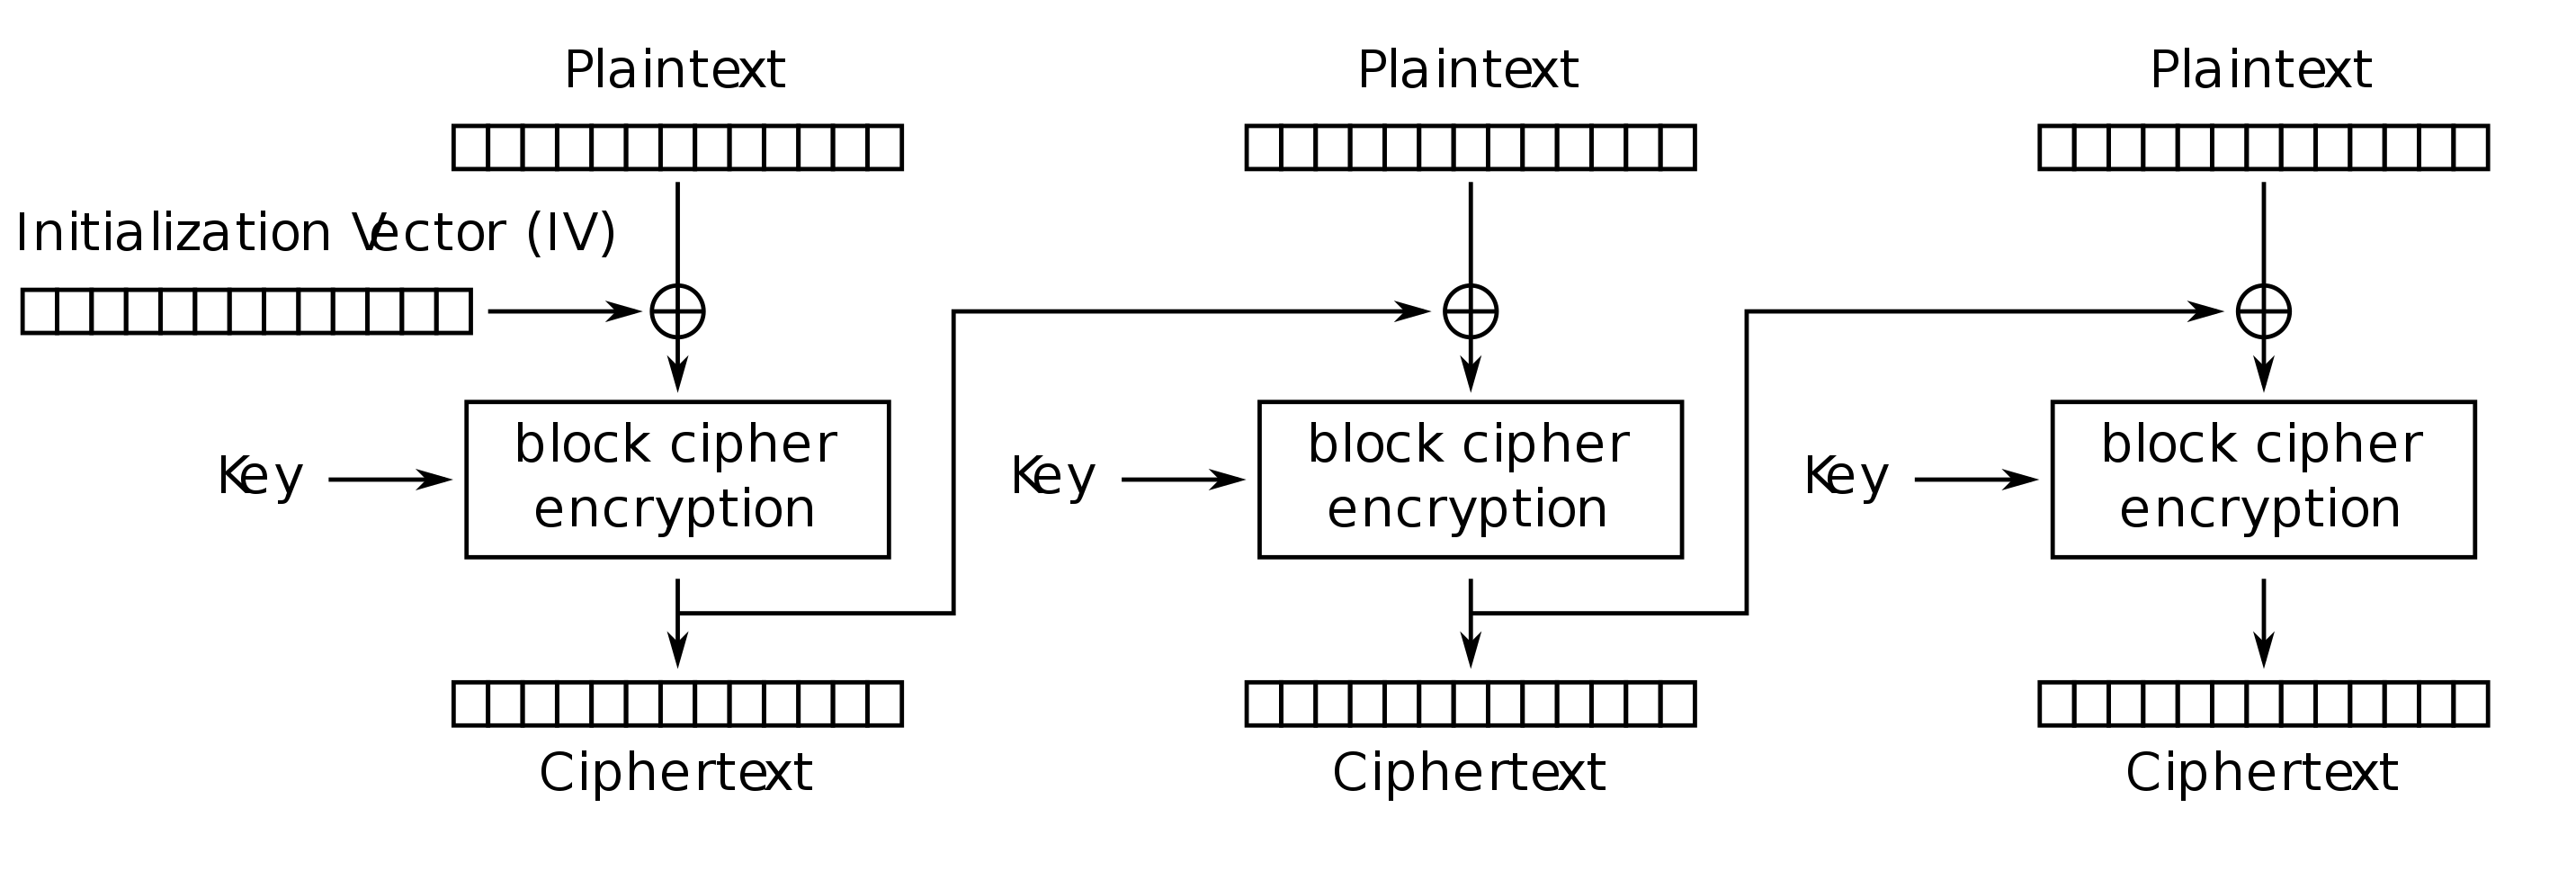
\includegraphics[width=0.7\textwidth]{img/CBC_encr.png}
    \centering
    \caption{CBC modalità cifratura}
    \label{fig:cbc_enc}
\end{figure}

Per quanto riguarda la decifratura del messaggio (figura \ref{fig:cbc_decr}), sarà sufficiente eseguire l'operazione inversa mettendo in Xor il cifrato del blocco precedente con l'output della funzione di decifratura, 
utilizzando all'inizio lo stesso vettore di inizializzazione (IV).

\begin{figure}[h!]
    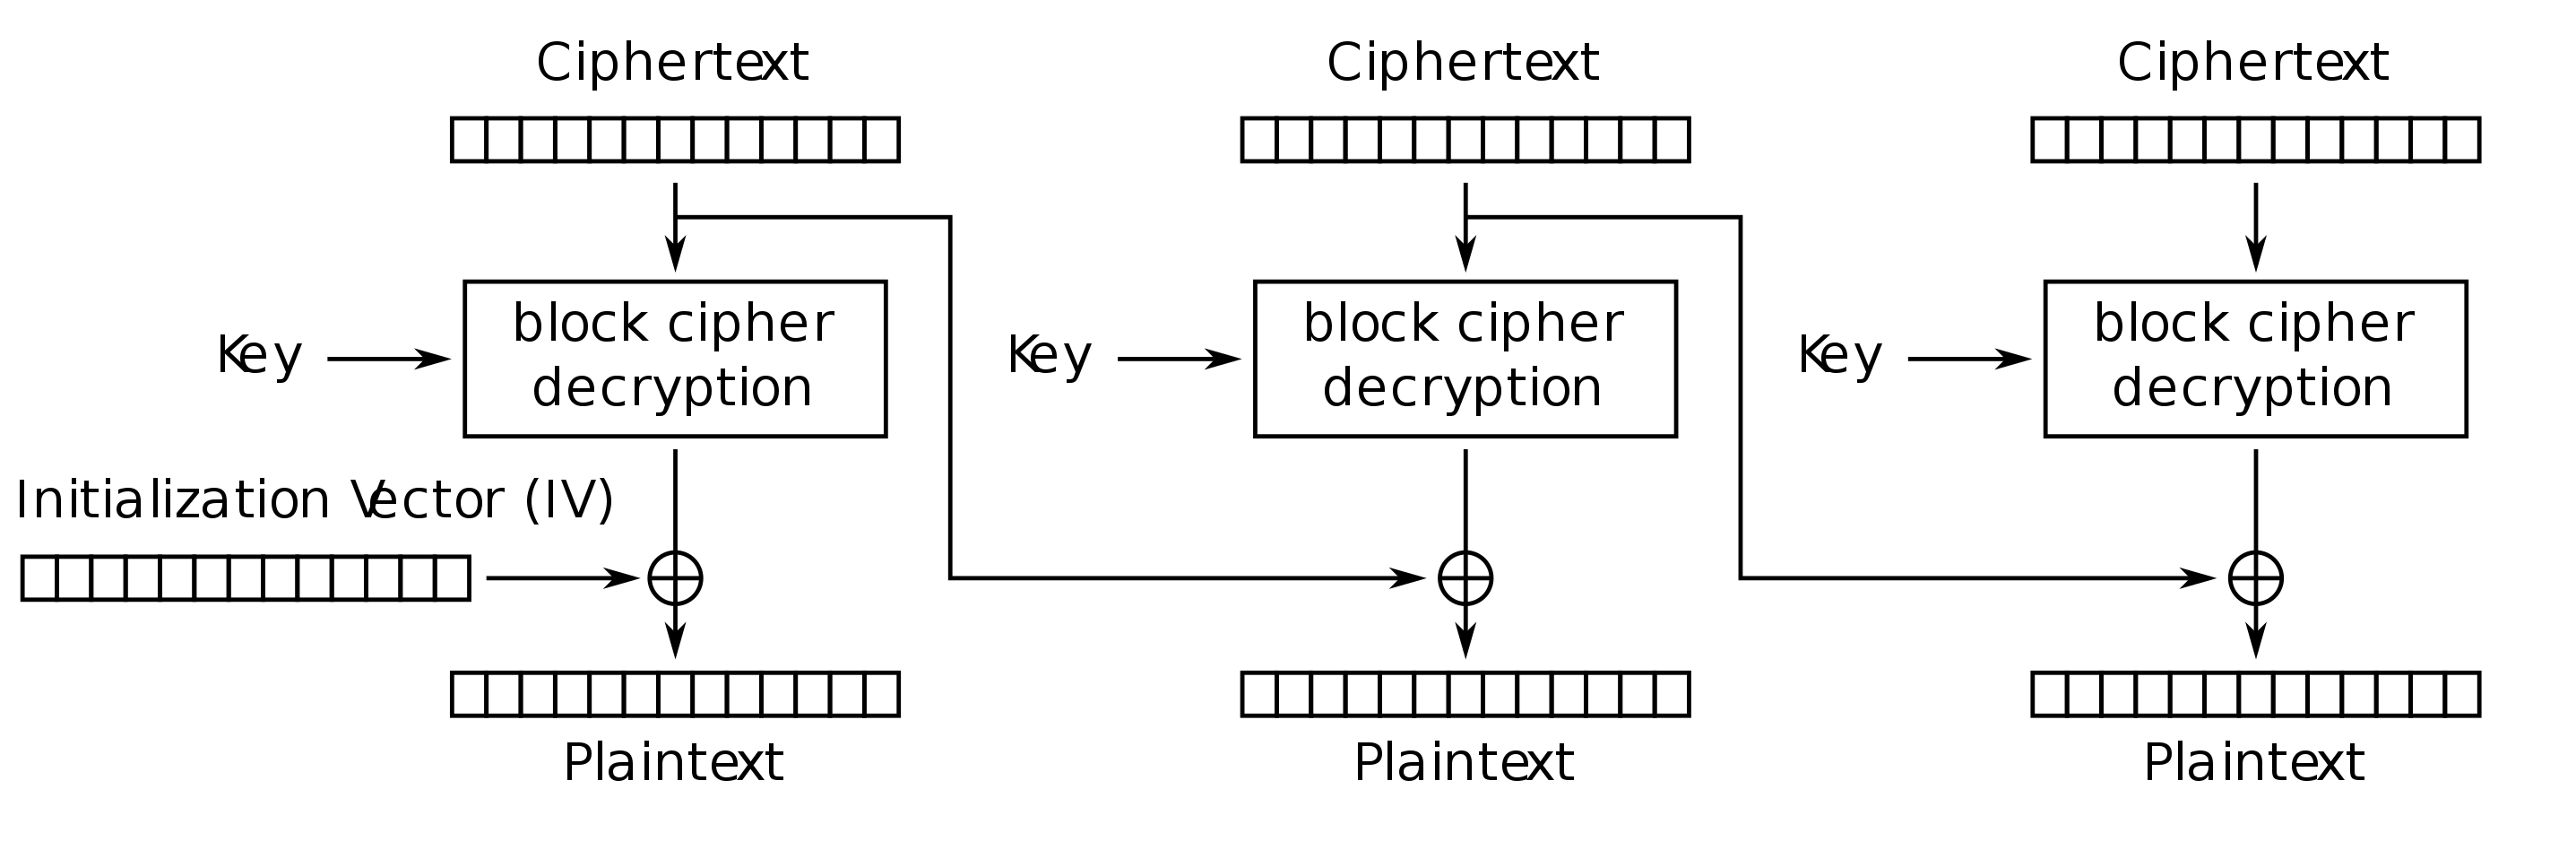
\includegraphics[width=0.7\textwidth]{img/CBC_decr.png}
    \centering
    \caption{CBC modalita decifratura}
    \label{fig:cbc_decr}
\end{figure}

\section{DES}
DES è un aloritmo di cifratura a chiave simmetrica, ovvero che usa la stessa chiave sia per cifrare che decifrare, 
la chiave deve essere scambiata su un canale sicuro dalle due parti coinvolte.
Lavora con blocchi in input di dimensione fissa da 64bit che tramite una serie di operazioni di trasformazione vengono 
portati in testo cifrato della stessa lunghezza
\section{Padding}
La cifratura a blocchi richiede una lunghezza fissa di bytes in ingresso, ma i messaggi da cifrare 
 non sono tutti multipli di quest'ultimap per questo, all'ultimo gruppo di bytes che non rispetta la dimensione viene aggiunto del padding finale.
Ci son diversi tipi di padding, quello che implementa DES è PKCS\#5, che consiste nel concatenare n bytes con valore pari al numero di bytes da
 aggiungere per arrivare alla dimensione del blocco. 
\\Quindi per esempio:

\begin{verbatim}
    01
    02 02
    03 03 03
    04 04 04 04
    05 05 05 05 05
    ...
\end{verbatim}
Questo metodo di padding supporta blocchi con massima lunghezza di 256byte, perchè un byte può rappresentare valori da 0 a 255.
Per esempio nel caso di DES dove la dimensione del blocco è di 64bit (8byte), un padding sarebbe:

\begin{verbatim}
    ... | AA AA AA AA AA AA AA AA | AA AA AA AA AA 03 03 03 |
\end{verbatim}
Nel caso in cui il massaggio sia invece  multplo esatto della lunghezza dei blocchi, per evitare di fare controlli aggiuntivi se il padding è da rimuovere o no, viene agiunto ugualmente un blocco intero di padding. In Questo modo in fase di decifratura il padding sarà sempre presente e sempre da rimuovere.
\section{Attacco padding Oracle}

L'attacco consiste nello sfruttare informazioni provenienti dalla correttezza del padding di un messaggio manipolato.
L'abilità di poter dare informazioni sulla correttezza del padding è data dal padding oracle che è un elmemento 
fondamentale dell'attacco senza il quale non è possibile procedere.
In (figura \ref{fig:attack_1}) è rappresenato un esempio di decifratura che aiuterà a spiegare la dinamica dell'attacco.
Per semplicità di rappresentazione vengono usati blocchi da 4 bytes ma il ragionamento può essere esteso a n bytes di blocchi.
I blocchi denominati con Dx rappresentano lo stato intermedio dopo la decifratura ma prima di eseguire l operazione di Xor, 
l' attacco si basa sul trovare proprio questo stato intermedio questo perchè:

\begin{verbatim}
   D = C ^ P 
   and 
   P = C ^ D
\end{verbatim}
C è conosciuto perchè è il testo cifrato, quindi trovato D possiamo ricavare il testo in chiaro P.

\begin{figure}[h!]
    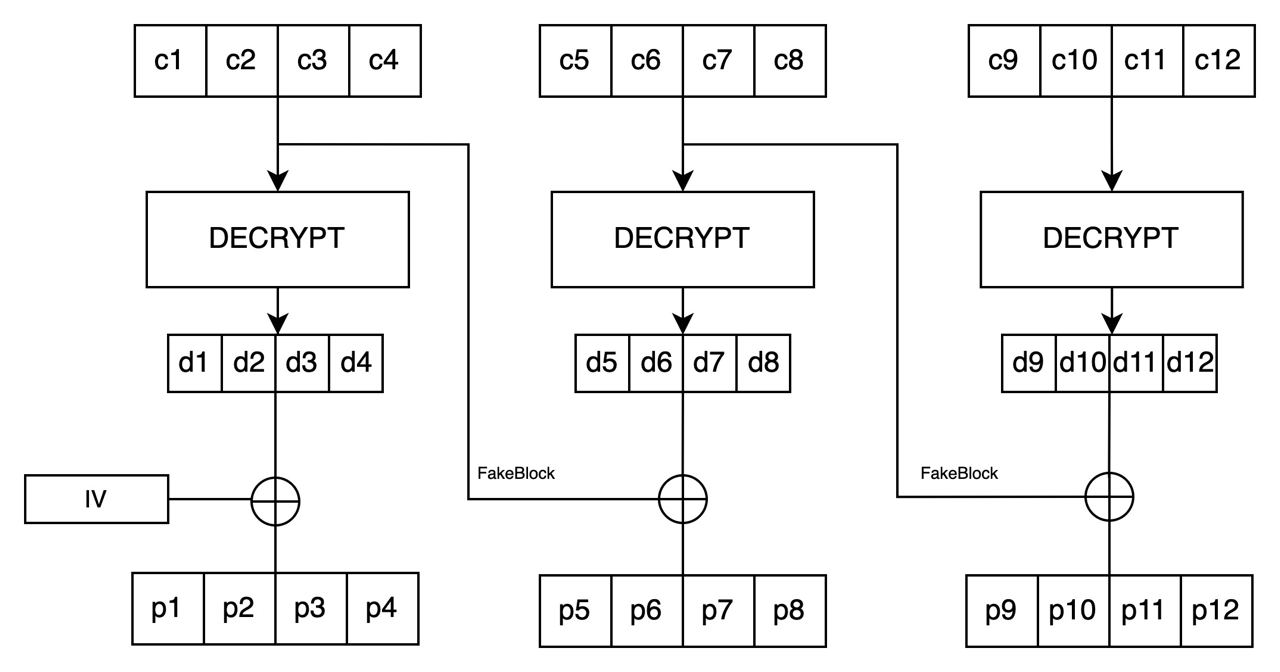
\includegraphics[width=0.8\textwidth]{img/attack.jpeg}
    \centering
    \caption{Spiegazione attacco}
    \label{fig:attack_1}
\end{figure}

\subsection{Manipolazione della cifratura}
Il padding oracle passato qualsiasi testo cifrato ci dirà se il padding è corretto o no, quindi ipotizzando di avere un padding 0x01 a P12 (P'12)
proviamo a trovare per quale byte a C8 otteniamo risposta positiva dal padding oracle.
Nella pratica (figura \ref{fig:attack_2}), facciamo variare da 0 a 255 il valore di C8, chiamandolo C'8, finchè il padding 
oracle non da risposta positiva, a quel punto abbiamo che:
\begin{verbatim}
    D12 = C'8 ^ P'12 
 \end{verbatim}
 \begin{figure}[h!]
    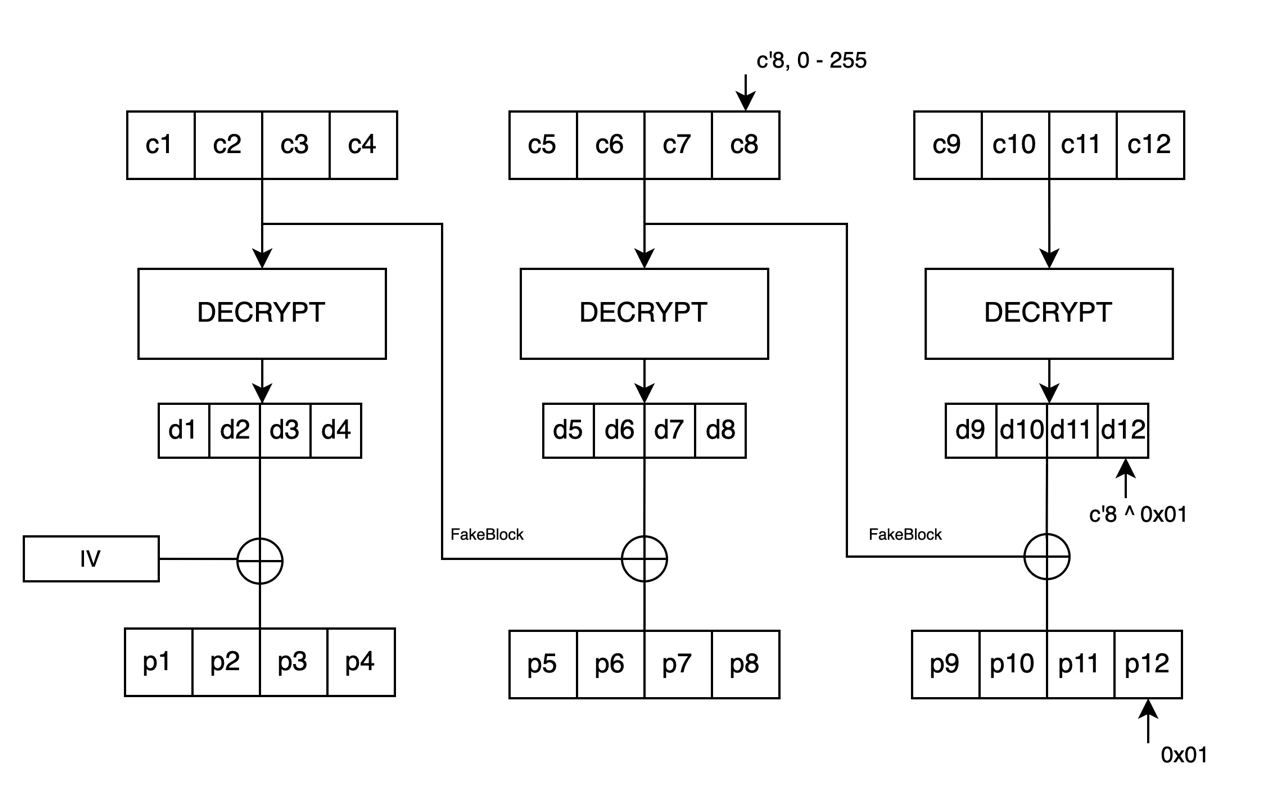
\includegraphics[width=0.8\textwidth]{img/attack_first_byte.jpeg}
    \centering
    \caption{Attacco al primo byte}
    \label{fig:attack_2}
\end{figure}
abbiamo trovato il valore di D, possiamo quindi procedere a trovare il l'effettivo valore di P12:
 \begin{verbatim}
    P'12 = D12 ^ C'8

    ma
    D12 = C8 ^ P12

    quindi

    P'12 = C8 ^ P12 ^ C'8
 \end{verbatim}
 Abbiamo che C8 è il byte originale del testo cifrato, C'8 il byte al quale il padding oracle ha risposto correttamente e P'12 il padding che abbiamo ipotizzato 0x01
 \begin{verbatim}
    P12 = C8 ^ 0x01 ^ C'8
 \end{verbatim}
abbiamo trovato il primo byte di testo in chiaro.
\subsection{Byte Successivi}
Il ragionamento che è stato fatto per un byte può essere ripotrato ai byte successivi, cambiando il padding corrispondente al numero di byte che sto manipolando.
Qundi  ora ipotizzo (figura \ref{fig:attack_2}) che il penultimo byte del testo in chiaro abbia padding 0x02 e cerco il valore c'7 che inviato al padding oracle dia validazione corretta.
Nel fare questa operazione però va cambiato anche il valore di c8 perchè l'intero padding deve essere corretto per non far fallire il padding oracle, e in questo caso il padding corretto lo 
si ha avendo anche p12 a 0x02, possedendo il valore di d12 però possiamo facilmente ricavare il corretto valore di c8
\begin{verbatim}
    C8 = D'12 ^ 0x02
 \end{verbatim}
 si continua con lo stesso procedimento fino alla fine del blocco.
\begin{figure}[h!]
    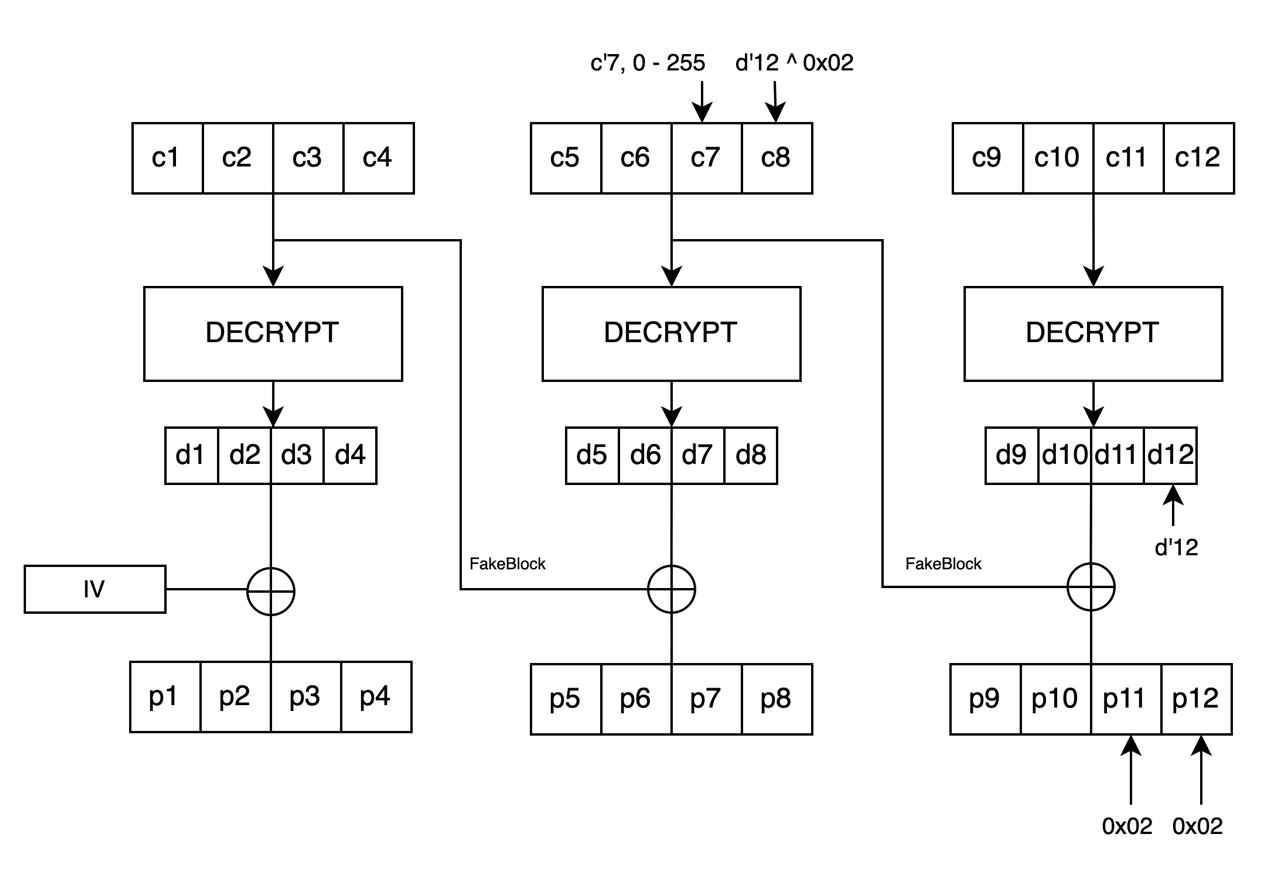
\includegraphics[width=0.8\textwidth]{img/attack_second_byte.jpeg}
    \centering
    \caption{Attacco al secondo byte}
    \label{fig:attack_3}
\end{figure}
\subsection{Blocchi Successivi}
Visto che la parte decifrata di un blocco dipende solo dal blocco precedente possiamo applicare il procedimento descritto ad ogni blocco rimanente tranne il primo, a meno di aver intercettato anche il vettore di inizializzazione.
Si ragiona come se il blocco da manipolare sia sempre il penutlimo agganciando il blocco successivo da mandare al padding oracle con il padding che riparte da 0x01 fino a rimepire la lunghezza del blocco.
\section{Prevenzione}
Il modo milgiore per proteggersi da un attacco padding oracle è non esporre un errore differente dal server nel caso in cui il padding non sia corretto.
Un ulteriore misura di precauzione che interviene ancora prima di decifrare i blocchi è introdurre una cifratura autenticata tramite l utilizzo di un hash che verifica l'integrità della cifratura andando a trovare se ci sono state delle manipolazioni. La parte cifrata viene inviata in coda al testo cifrato